\section{Task}
Several tasks has been identified in our project. In the following table we can find three categories: one that labels the tasks, one for the description and the last one for the completion state to each task.

\begin{center}
	\begin{tabulary}{\linewidth\tymin=70pt}{Y{2cm}|Y{6cm}|Y{2.25cm}}
		\textbf{Task} & \textbf{Description} & \textbf{Completed?}\\ \hline
		T1a & RASD - Writing & Yes \\ \hline
		T1b & RASD - Presentation & Yes \\ \hline
		T2a & DD - Writing & Yes \\ \hline
		T2b & DD - Presentation & Yes \\ \hline
		T3 & ITPD - Writing & Yes \\ \hline
		T4 & PPD - Writing & Yes \\ \hline
		T5 & Implementation & No \\ \hline
		T6 & Unit Testing & No \\ \hline
		T7 & Integration Testing & No \\ \hline
		T8 & System Testing & No \\ \hline
		T9 & User Acceptance - Alpha Testing & No \\ \hline
		T10 & User Acceptance - Beta Testing & No \\ \hline
		T11 & Release To Market & No \\
	\end{tabulary}
\end{center}

\section{Schedule}
Below there are represented a table and a diagram that show how the time has been divided between the various phase of the software life cycle ; the result is then more clear in Gantt chart.
The table identifies:

\begin{itemize}
  \item The date in which the given task starts,
  \item The date in which the given task ends,
  \item The interval in [\textbf{day}] that separates the starting date from the ending date
\end{itemize}

\begin{center}
	\begin{tabulary}{\linewidth\tymin=70pt}{Y{1cm}|Y{3cm}|Y{3cm}|Y{1.7cm}}
		\textbf{Task} & \textbf{Start} & \textbf{End} & \textbf{Interval} \\ \hline
		T1a & 16/10/2016 & 13/11/2016 & 28\\ \hline
		T1b & 16/11/2016 & 16/11/2016 & 1\\ \hline
		T2a & 17/11/2016 & 11/12/2016 & 24\\ \hline
		T2b & 14/12/2016 & 14/12/2016 & 1\\ \hline
		T3 & 09/01/2017 & 15/01/2017 & 6\\ \hline
		T4 & 16/01/2017 & 22/02/2017 & 6\\ \hline
		T5 & 04/02/2017 & 30/05/2017 & 117\\ \hline
		T6 & 31/05/2017 & 29/06/2017 & 29\\ \hline
		T7 & 30/06/2017 & 28/07/2017 & 28\\ \hline
		T8 & 29/07/2017 & 29/08/2017 & 31\\ \hline
		T9 & 30/08/2017 & 27/09/2017 & 28\\ \hline
		T10 & 28/09/2017 & 26/10/2017 & 28\\ \hline
		T11 & 27/10/2017 & 27/10/2017 & 1\\
	\end{tabulary}
\end{center}

\section{Gant Diagram}
Here is built a Gantt Diagram showing the schedule chosen for \PowerEnJoy{} project tasks

\begin{center}
  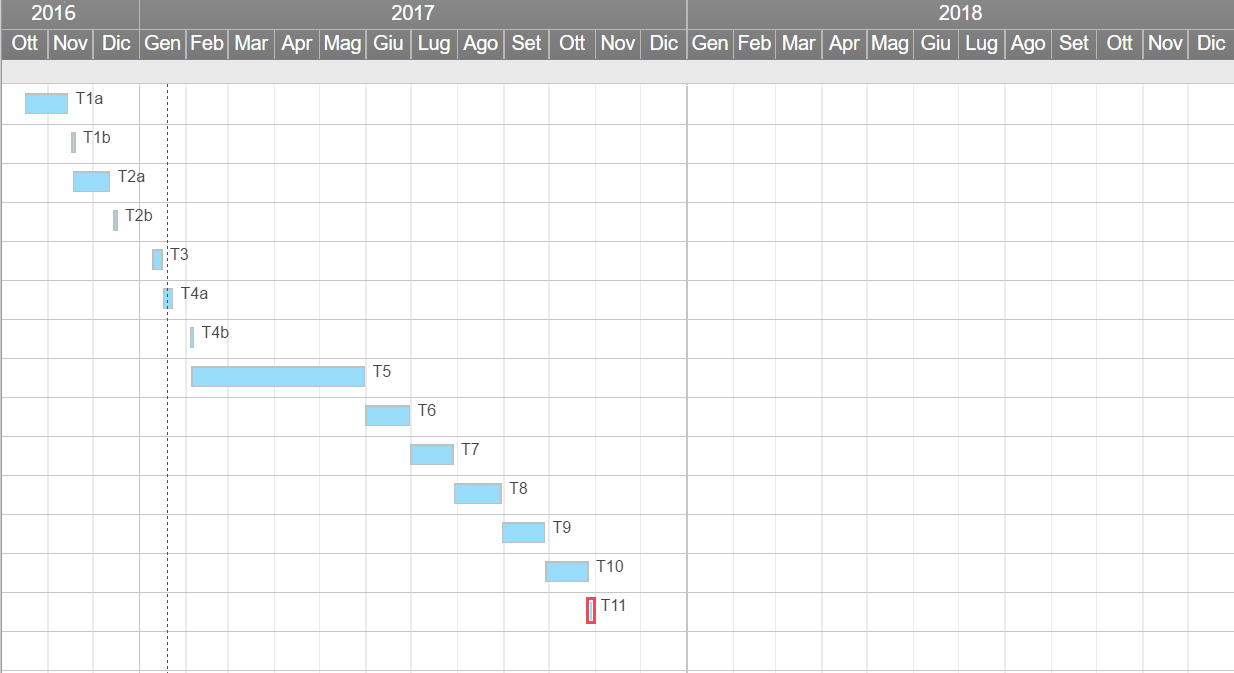
\includegraphics[width=\textwidth]{Resources/GanttDiagram.PNG}
  \captionof{figure}{Gant Diagram}
  \label{Gant Diagram}
\end{center}
